\documentclass[11pt]{article}

\usepackage{fancyhdr}
\usepackage{verbatim}
\usepackage{amsfonts,amsmath,graphicx,color,epsfig}
\usepackage[latin1]{inputenc}

\fontsize{12}{15}

\textwidth 16cm
%\oddsidemargin 0cm
%\textheight 21cm
%\topmargin -1.4cm
%\headsep 2cm

\setlength{\oddsidemargin}{0in}
\setlength{\evensidemargin}{0in}
% \setlength{\textwidth}{6.1in}
\setlength{\topmargin}{0in}
\setlength{\textheight}{8.5in}

%%%%%%%%%%%%%%%%%%%%%
%%% headings
%%%%%%%%%%%%%%%%%%%%%
%
%\pagestyle{fancyplain}
%
%\addtolength{\headheight}{3pt}
%\renewcommand{\sectionmark}[1]{\markright{{ \thesection}  { #1}}}
%
%\fancyhead[LE]{{\bf\thepage}}
%\fancyhead[RE]{\leftmark}
%
%\fancyhead[RO]{{\bf\thepage}}
%\fancyhead[LO]{\rightmark}
%\cfoot{}
%
%\fancypagestyle{white}{%
%\fancyhf{} %
%\fancyhead[LE]{{\bf\thepage}}
%\fancyhead[RO]{{\bf\thepage}}
%\cfoot{}
%}

\newcommand{\ie}{{\em i.e. }}
\newcommand{\eg}{{\em e.g. }}
\newcommand{\un}{{\bf 1}}

\newcommand{\bz}{{\bf z}}
\newcommand{\bL}{{\bf \Lambda}}
\newcommand{\bl}{{\bf \lambda}}
\newcommand{\bD}{{\mathcal{D}}}
\newcommand{\bT}{{\mathcal{T}}}
\newcommand{\bR}{{\mathbb{R}}}
\newcommand{\bP}{{\mathbb{P}}}
\newcommand{\bE}{{\mathbb{E}}}
\newcommand{\bN}{{\cal N}}
\newcommand{\lck}{\left\lbrack}
\newcommand{\rck}{\right\rbrack}
\newcommand{\lce}{\left\lbrace}
\newcommand{\rce}{\right\rbrace}
\newcommand{\var}{\text{Var}}
\newcommand{\cov}{\text{Cov}}

\newcommand{\dint}{{\int \!\!\!\!\! \int}}
\newcommand{\Un}{{\bf 1}}
\newcommand{\dd}{\, \mbox{d}}

\definecolor{orange}{cmyk}{0,0.5,0.8,0}
\definecolor{jaune}{cmyk}{0,0,1,0}
\definecolor{rouge}{rgb}{1,0,.2}
\definecolor{bleu}{rgb}{0,0,1}
\definecolor{violet}{rgb}{0.6,0,.8}
\definecolor{vert}{rgb}{.2,.6,.2}
\definecolor{turquoise}{cmyk}{0.8,0,0,0}
\definecolor{gris}{rgb}{0.3,0.3,0.3}

\renewcommand{\baselinestretch}{1}

\begin{document}
\graphicspath{{./figures/}}


\begin{center}
  {\Large {\bf STPP: Plotting, simulating and analysing Spatio-Temporal Point Patterns}}

  \bigskip

  Edith {\sc Gabriel}$^*$, Barry {\sc Rowlingson}$�$ and Peter J {\sc Diggle}$�$

	\bigskip
	
	$^*$\textit{Universit� d'Avignon, France},
	$�$\textit{Lancaster University, UK}.

	\bigskip

  \today
\end{center}

\bigskip
\bigskip

\begin{center}
\begin{minipage}[c]{12cm}
{\textbf{Abstract:} \verb#stpp# is an R package for analysing,  simulating
and displaying space-time point patterns. It covers many of the models
encountered in applications of point process methods to the study of spatio-temporal phenomena and propose an estimator of the space-time inhomogeneous $K$-function. In this paper we describe space-time point processes and introduce the package \verb#stpp# to new users.

\bigskip

\textit{Keywords:} epidemiology; inhomogeneous point patterns; spatial statistics;
space-time point processes.}
\end{minipage}
\end{center}

\bigskip
\bigskip

\section{Introduction}

A spatial point pattern is a set of data taking the form of a set of locations, irregularly
distributed within a study region $S$, at which events
have been recorded, for example the locations of trees in a naturally regenerated forest
(Diggle, 2003).

An observed spatial point pattern can be modelled as a realisation of
a spatial stochastic process represented by a set of random variables:
$Y(S_m), S_m \subset S$, where $Y(S_m)$ is the number of events
occurring in a sub-region $S_m$ of $S$.
Simulation of spatial point processes is mainly implemented in the R packages
 \verb#spatstat# (Baddeley and Turner, 2005) and \verb#splancs# (Rowlingson and Diggle, 1993).

Many spatial processes of scientific interest also have a temporal component
that may need to be considered when modelling the
underlying phenomenon (\eg distribution of cases for a disease or
assessment of risk of air pollution).
Spatio-temporal point processes, rather than purely spatial point processes,
must then be considered as potential models.
There is an extensive literature on the analysis of point process data in time
(e.g. Cox and Isham, 1980; Daley and Vere-Jones, 2003)
and in space (e.g. {Cressie, 1991; Diggle, 2003; M{\o}ller and Waagepetersen,
2003).
Generic methods for the analysis of spatio-temporal point processes are less well
established; see for example Diggle, 2006 and Gabriel and Diggle, 2009). There
is, however, an
extensive literature on the use of point process models in
the specific field of seismology; see, for example,
Zhuang, Ogata and Vere-Jones (2002) and references therein.

In this paper we first define such processes. Then, we present models for
spatio-temporal point processes, some algorithms for their simulation, and statistical tools for their analysis.


\section{Spatio-Temporal Point Processes}

The events of  a spatio-temporal point process
form  a countable set of points, ${\cal P} = \{(s_{i},t_i):i=1,2,...\}$,
in which $s_{i} \in S \subset \bR^2$ is the location
and $t_i \in T \subset \bR$ is the time of occurrence of the $i$th event.
In the following, $Y(A)$
denotes the number of events in a region $A$.


\subsection{First-order and second-order properties}
\label{subsec:intensity}

First-order properties describe the way in which the expected value of the
process varies across the spatio-temporal domain of observation, $S \times T$,
where typical $S$ is a polygon and $T$ a single closed interval.
These properties are described by the intensity, $\lambda(s,t)$,
of the process,
\begin{equation*}
  \lambda(s,t) = \lim_{|d s| \to 0, |dt| \to 0}
  \frac{\bE \lck Y(d s, dt) \rck}{|d s| |dt|},
\end{equation*}
where $d s$ defines a small spatial region around the point $s$, $|d s|$
is its area, $dt$ is a small interval containing time $t$, $|dt|$ is the
length of this interval and $Y(ds, dt)$ refers to the number of events
in $d s$ in the interval of time $dt$. Thus, informally,
$\lambda(s,t)$ is the mean number of events per unit volume at the location
$(s,t)$.

Second-order properties define one aspect of
 spatio-temporal dependence by describing the
relationship between numbers of events in pairs of subregions within
$S \times T$.
The second-order spatio-temporal intensity is defined by:
\begin{equation*}
  \lambda_2 \big((s_{i},t_i),(s_{j},t_j)\big) = \lim_{|D{i}|,
    |D_{j}| \to 0} \frac{\bE \lck Y(D_{i}) Y(D_{j}) \rck}
  {|D_{i}||D_{j}| },
\end{equation*}
where $D_{i} = d s_{i} \times dt_i$ and $D_{j} = d s_{j}
\times dt_j$ are small cylinders containing the points $(s_{i},t_i)$
and $(s_{j},t_j)$ respectively.

Other, essentially equivalent, descriptors of second-order properties include the
covariance density,
\begin{equation*}
\gamma\big((s_{i},t_i),(s_{j},t_j)\big) =  \lambda_2 \big((s_{i},t_i),(s_{j},t_j)\big) - \lambda(s_i,t_i) \lambda(s_j,t_j)
\end{equation*}
and the radial distribution function or
point-pair correlation function
\begin{equation*}
  g\big( (s_i,t_i), (s_j,t_j) \big) = \frac{\lambda_2 \big((s_{i},t_i),
    (s_{j},t_j)\big)} {\lambda (s_i,t_i) \lambda (s_j,t_j)}.
\end{equation*}
(Cressie, 1991; Diggle, 2003).
The covariance density is the point process analogue of the covariance function of a real-valued
stochastic process.
The pair correlation function can be interpreted informally as the standardised
probability density that an event occurs in each of two small volumes centred on the
points $(s_i,t_i)$ and $(s_j,t_j)$. For a spatio-temporal Poisson process (to be defined formally
in Section \ref{sec:Poisson}), the covariance density is identically zero
and the pair correlation function is identically 1. Larger or smaller values
than these benchmarks therefore indicate informally how much more or less likely it is
that a pair of events
will occur at the specified
locations than in a Poisson process with the same intensity.

\subsection{Stationarity}

\noindent
{\em Space-time first-order and second-order stationarity}

\medskip

\noindent
A spatio-temporal point process $\lce (s,t), s \in S, t \in T \rce$
is first-order and second-order stationary:
\begin{itemize}
\item [{\scriptsize $\bullet$}] in space, if:
$\lambda(t|s) \equiv \lambda(t) \ \text{ and } \
\lambda_2 \big(s_{i},s_j|t \big) = \lambda_2(s_{i}-s_{j},t).$

\item [{\scriptsize $\bullet$}] in time, if:
$\lambda(s|t) \equiv \lambda(s) \ \text{ and } \
\lambda_2 \big(t_i,t_j|s \big) = \lambda_2(s,t_i-t_{j}).$

\item [{\scriptsize $\bullet$}] in both space and time, if:
$\lambda(s,t) = \lambda \ \text{ and } \ \lambda_2 \big((s_{i},t_i),
(s_{j},t_j)\big) = \lambda_2(s_{i}-s_{j},t_i-t_j).$
\end{itemize}
If the process is also isotropic, $\lambda_2 \big((s_{i},t_i),
(s_{j},t_j)\big) = \lambda_2 (u,v)$, where $u= \| s_{i}-s_{j} \|$
and $v = |t_i-t_j|$.


\bigskip

\noindent
{\em Space-time second-order intensity reweighted stationarity}

\medskip

\noindent
A spatio-temporal point process is second-order intensity reweighted
stationary and isotropic if its intensity function is bounded away from
zero and its pair correlation function
depends only on the spatio-temporal difference vector $(u,v)$ (Baddeley, M{\o}ller and Waagepetersen, 2000).

\subsection{Separability}

%\noindent
%{\em First-order and second-order separability}

%\medskip

\noindent
A spatio-temporal point process is first-order separable if its intensity
$\lambda(s,t)$ can be factorised as
$$\lambda(s,t) = m(s) \mu(t), \ \text{for all } (s,t) \in S \times T.$$

\noindent
Second-order separability of a spatio-temporal
point process is typically defined only when the process is stationary,
in which separability  means that the covariance density $\gamma(u,v) = \lambda_2(u,v) - \lambda^2$
factorises as
\begin{equation*}
\gamma(u,v) = \gamma_s(u) \gamma_t(v)
\end{equation*}
Note that in general, second-order separability is implied by, but does
not imply, independence of the spatial and temporal component processes.
Covariance separability of a process does not imply separability. However, a Poisson process has
independent components if and only if it is first-order separable
of the process itself.



\subsection{Static and dynamic plotting of spatio-temporal point process data}

The most effective form of display for a spatio-temporal point process
data is an animation, repeated viewing of which may yield insights
that are not evident in static displays. Nevertheless, static displays are
sometime useful summaries. The \verb#sttp# package includes four display functions
that we illustrate using data on the locations and times (dates of reporting) of outbreaks
of foot-and-mouth disease (FMD), a severe, highly communicable viral
disease of farm livestock, during the UK 2001 FMD epidemic.

The dataset \verb#fmd#, included in \verb#sttp# contains a three-column matrix
of spatial locations and reported days (counted from 1st February) of FMD outbreaks in
the county of
Cumbria. Figure~\ref{fig:fmd1} shows a static display of the data consisting
of locations in the left-hand panel and
the cumulative distribution of the times in the right-hand panel. The left-hand panel shows a
very uneven distribution which in the context of this data-set is of limited interest without
knowledge of the spatial distribution of all of the farms at risk.
The right-hand panel shows
the characteristic S-shape of an epidemic process.
Such plot can be obtained in a single command after converting the dataset into an
object of class `stpp' as follows.
\begin{verbatim}
> library(stpp)
> data(fmd)
> data(northcumbria)
> fmd=as.3dpoints(fmd)
> plot(fmd, s.region=northcumbria)
\end{verbatim}
\begin{figure}
\centering
%\epsfig{file=fmdxy.eps,width=5cm,height=5cm}
%\epsfig{file=fmdt.eps,width=5cm,height=5cm}
\caption{Static two-panel plot of
data from the 2001 UK FMD epidemic in the county of Cumbria.}
\label{fig:fmd1}
\end{figure}

Figure \ref{fig:fmd2} shows an alternative static display in which the time is treated as a quantitative mark
attached to each location, and the locations are plotted with the size and/or colour of the plotting
symbol determined by the value of the mark.
\begin{figure}
\centering
%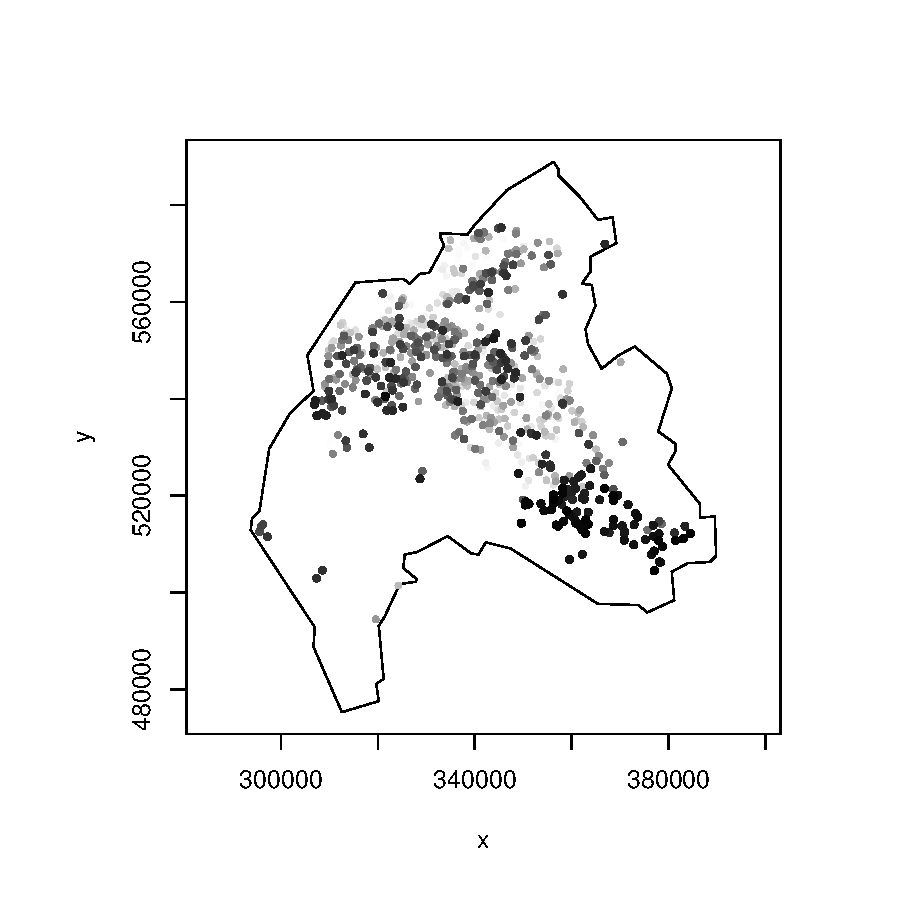
\epsfig{file=fmd.eps,width=6cm,height=6cm}
\caption{Static plot of
data from the 2001 UK FMD epidemic. Time is treated as a quantitative mark; light grey/small dots correspond to the oldest events and dark grey/large dots correspond to the most recent events.}
\label{fig:fmd2}
\end{figure}
Such plot can be obtained as follows.
\begin{verbatim}
> plot(fmd, s.region=northcumbria, pch=19, mark=TRUE)
\end{verbatim}

\noindent
The function \verb#animation# provides an animation of a space-time point
pattern.
\begin{verbatim}
> animation(fmd,runtime=10,cex=0.5,s.region=northcumbria)
\end{verbatim}
The approximate running time of the animation (in seconds) is set through the \verb#runtime#
parameter, although the animation may actually run more slowly than this, depending on the
size of the data-set and the hardware configuration.
If \verb#runtime=NULL#, the animation is displayed as quickly as the data-set and hardware configuration
allow.

A second form of dynamic display is provided by
the \verb#stan# function. This enables dynamic
highlighting of time slices controlled by two arguments set by using sliders: when the 'time'
 slider is set to $T$ and the 'width' slider to $W$, highlighted points are
 those whose time coordinate $t$ satisfies $T-W < t <T$.
Plotting of individual locations is controlled with the `{\tt states}' parameter. This is a
list of length three specifying how locations whose associated times
 fall before, within and after the time window are displayed. The use of sliders allows the
 user to track backward or forward in time at will.
\begin{verbatim}
> library(rgl)
> library(rpanel)
> stan(fmd, twid=1, bgpoly=northcumbria, bgframe=FALSE)
\end{verbatim}
Repeated  viewing of either of the graphic displays
shows two main features of the epidemic. Firstly,
there was a progressive movement of the epidemic's focus from its origin in the north of the
county to the west, and later to the south-east. Secondly, the pattern consists predominantly
of spatio-temporal
spread  between neighboring
farms, but with occasional and apparently spontaneous infections occurring
remotely from previously infected areas.



\subsection{Space-time inhomogeneous $K$-function}

\noindent
For a second-order intensity reweighted stationary, isotropic
spatio-temporal point process, the space-time inhomogeneous $K$-function (STIK-function) defined by Gabriel and Diggle (2009) is
  $$K_{ST}(u,v) =  2 \pi \int_0^v \int_0^u g(u',v') u' \dd u' \dd v',$$
  where $g(u,v) = \lambda_2(u,v) / \left( \lambda(s,t) \lambda (s',t')
  \right)$, $u = \| s-s' \|$ and $v = |t - t'|$.
They also provide a second definition which considers both past and future events,
$$K_{ST}^*(u,v) = 2 \pi \int_{-v}^v \int_0^u g(u',v') u' \dd u' \dd v'.$$
%as used in M{\o}ller and Ghorbani (2011).

\noindent
Being an alternative characterization of the second-order properties of a point process, the STIK function can be used as a measure of
the spatio-temporal aggregation or regularity of clustering. Indeed, for any inhomogeneous spatio-temporal Poisson process (see section~\ref{sec:Poisson}) with intensity bounded away from zero, $K_{ST}(u,v) = \pi u^2 v$. Values of $K_{ST}(u,v)$ greater than $\pi u^2 v$ indicate aggregation at spatial and temporal separations less than $u$ and $v$, whilst $K_{ST}(u,v) < \pi u^2 v$ indicates regularity.
It can also be used to test for space-time clustering and space-time interaction (Gabriel and Diggle, 2009; M{\o}ller and Ghorbani, 2011).

\noindent
The function \verb#STIKhat# provides a non parametric estimation of the STIK function (as defined in Gabriel and Diggle, 2009).
It has been applied to FMD data under the assumption of separability of the spatio-temporal intensity. 
\begin{verbatim}
> FMD=as.3dpoints(fmd[,1]/1000,fmd[,2]/1000,fmd[,3])

> # estimation of the temporal intensity
> M=density(FMD[,3],kernel="gaussian",n=200)
> mut=M$y[FMD[,3]]*dim(fmd)[1]

> # estimation of the spatial intensity
> h = mse2d(pts=FMD[,1:2], poly=northcumbria/1000, nsmse=100, range=5)
> hs=h$h[h$mse==min(h$mse)]
> require(spatialkernel)
> mhat <- lambdahat(pts=as.points(FMD[,1:2]), h=hs, gpts=as.points(FMD[,1:2]),
          poly = northcumbria/1000, edge = TRUE)$lambda

> # estimation of the STIK function
> u <- seq(0,10,by=1)
> v <- seq(0,15,by=1)
> stik <- STIKhat(xyt=FMD, s.region=northcumbria/1000,t.region=c(1,200),
          lambda=mhat*mut/dim(fmd)[1], dist=u, times=v, infectious=T)
\end{verbatim}
We can plot the estimate by using the function \verb#plotK#.
\begin{verbatim}
> # plotting the estimation
> plotK(stik)
> plotK(stik,persp=T,theta=-65,phi=35)
\end{verbatim}
Figure~\ref{fig:stik} shows such plot for FMD data where $u$ gives distances in kilometers and $v$ times in days.
\begin{figure}
\centering
%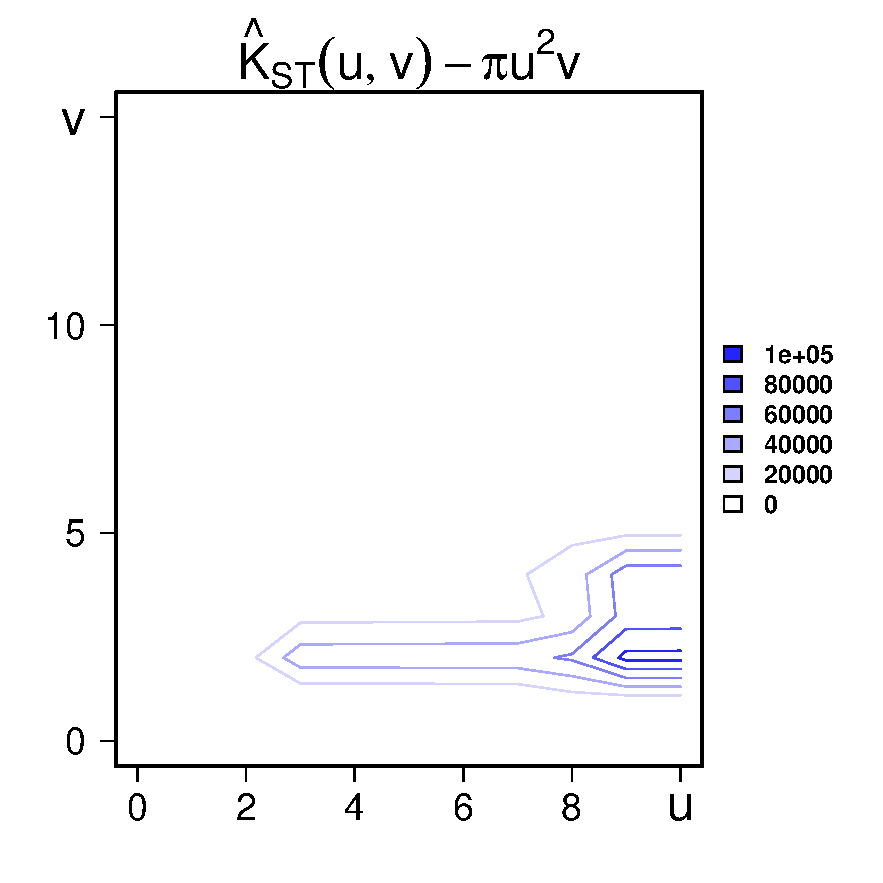
\epsfig{file=stik.contour.eps,width=6cm,height=6cm}
%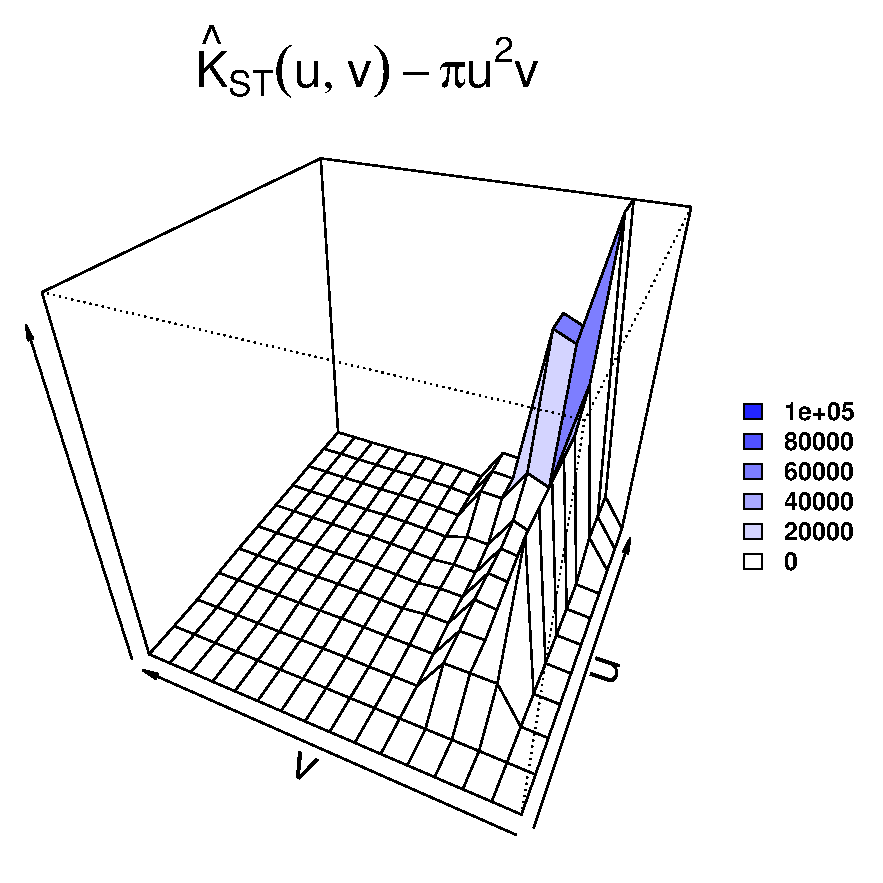
\epsfig{file=stik.persp.eps,width=6cm,height=6cm}
\caption{Contour plot (left) and perspective plot (right) of the STIK function estimated from FMD data.}
\label{fig:stik}
\end{figure}







\section{Models}

\subsection{Poisson process} \label{sec:Poisson}

\subsubsection*{Homogeneous Poisson process}

The homogeneous Poisson process represents the simplest possible stochastic
mechanism for the generation of spatio-temporal point patterns. It is rarely plausible as a
model for data, but provides a benchmark of complete spatio-temporal randomness (CSTR). Informally,
in a realisation of a homogenous Poisson process on any spatio-temporal region
$S \times T$, the events form an independent random sample from the uniform distribution on
$S \times T$. More formally,
the homogeneous Poisson process is defined by the following postulates,
which correspond to the definition of CSTR:
\begin{enumerate}
\item For some $\lambda > 0$, the number $Y(S \times T)$ of events
within the region $S \times T$ follows a Poisson distribution with
mean $\lambda |S| T$, where $T$ is the length of the time interval $T$.
\item Given $Y(S \times T) = n$, the $n$ events in $S \times T$
form an independent random sample from the uniform distribution on
$S \times T$.
\end{enumerate}

\noindent
The first-order and second-order intensities of a homogeneous Poisson process
reduce to constants, $\lambda(s,t) = \lambda$ and $\lambda_2 \big((s_{i},t_i),(s_{j},t_j)\big) = \lambda^2$.
Hence, as stated in Section \ref{subsec:intensity}, the covariance density is identically zero, the pair correlation function identically 1, and the STIK function is $K_{ST}(u,v) = \pi u^2 v$.

\medskip

\noindent \underline{\noindent {\em Simulation}}

\medskip

\noindent
To generate a homogeneous Poisson point pattern in $S \times T$ a two step
procedure can be used.
{\em
\begin{enumerate}
\item Simulate the number of events $n=Y(S \times T)$ occurring in
  $S \times T$ according to a Poisson distribution with mean
  $\lambda |S| T$.
\item Sample each of the $n$ locations and $n$ times according to a uniform
  distribution on $S$ and on $T$ respectively.
\end{enumerate} }


\subsubsection*{Inhomogeneous Poisson process}

The inhomogeneous Poisson process is the simplest non-stationary
point process. It is obtained replacing the constant intensity $\lambda$
of a homogeneous Poisson process by a spatially and/or temporally varying
intensity function $\lambda(s,t)$. Inhomogeneous Poisson processes are
defined by the following postulates:
\begin{enumerate}
\item The number $Y(S \times T)$ of events within the region $S \times
  T$ follows a Poisson distribution with mean $\int_S \int_T
  \lambda(s,t) \dd t \dd s$.
\item Given $Y(S \times T) = n$, the $n$ events in $S \times T$ form
  an independent random sample from distribution on $S \times T$ with
  probability density function $f(s,t) = \lambda(s,t) / \int_S \int_T
  \lambda(s',t') \dd t' \dd s'$.
\end{enumerate}

\noindent
For any Poisson process, with intensity $\lambda(s,t)$, the second-order intensity
is $\lambda_2\big((s_i,t_i),(s_j,t_j)\big) = \lambda(s_i,t_i) \lambda(s_j,t_j)$, hence the
covariance density is identically zero, the pair correlation function identically 1, and the STIK fucntion $K_{ST}(u,v) = \pi u^2 v$ as in
the homogeneous case.

\medskip

\noindent \underline{{\em Simulation}}

\medskip

\noindent
To generate a realisation of an inhomogeneous Poisson process in $S \times T$,
we use a
thinning algorithm as follows.
For a given intensity function $\lambda(s,t)$:
{\em \begin{enumerate}
  \item Define an upper bound $\lambda_{max}$ for the intensity
    function $\lambda(s,t)$.
  \item Simulate a homogeneous Poisson process with intensity $\lambda_{max}$.
  \item ``Thin'' the simulated process according to the following way:
    \begin{enumerate}
    \item Compute $p=\lambda(s,t)/\lambda_{max}$ for each point $(s,t)$
      of the homogeneous Poisson process.
    \item Generate a sample $u$ from the uniform distribution on $(0,1)$.
    \item Retain the locations for which $u \leq p$.
    \end{enumerate}
  \end{enumerate} }


\subsubsection*{Examples}

Poisson processes are simulated by the function \verb#rpp#.
Realisations are simulated in a region $S \times T$, where $S$ is a polygon
and $T$ is an interval; default is the unit cube.
For a homogeneous Poisson process, the intensity is specified by a constant.
For example, the sequence of commands
\begin{verbatim}
> hpp1 = rpp(lambda=200, nsim=5, replace=FALSE)
> stan(hpp1$xyt[[2]])
\end{verbatim}
generates five realisations of the Poisson process with intensity $\lambda=200$
in the unit cube and displays the second realisation.

The sequence of commands
\begin{verbatim}
> data(northcumbria)
> hpp2 = rpp(npoints=1000, s.region=northcumbria, t.region=c(1,500),
 discrete.time=TRUE)
> polymap(northcumbria)
> animation(hpp2$xyt, s.region=hpp2$s.region)
\end{verbatim}
generates and displays a realisation of the Poisson process with intensity
$\lambda =1000/(|S|T)$ conditioned to produce exactly 1000 points
in the region $S \times T$, where
$S$ is the county of Cumbria and $T=[1,500]$. The argument \verb#npoints#
specifies the fixed value of the number of events to be generated.
Simulated times are restricted to integers (set by
the \verb#discrete.time# parameter), and coincident times are allowed
(set by the \verb#replace# argument).

The function \verb#rpp# can also generate realisations of inhomogeneous
Poisson processes. The intensity is then specified either by a function of the coordinates
and times, $\lambda(x,y,t,...)$, or by a pixel image if  the \verb#lambda# parameter
is a character. For example,
the sequence of commands
\begin{verbatim}
> lbda1 = function(x,y,t,a){a*exp(-4*y) * exp(-2*t)}
> ipp1 = rpp(lambda=lbda1, npoints=200, a=1600/((1-exp(-4))*(1-exp(-2))))
> stan(ipp1$xyt)
\end{verbatim}
generates $200$ points of the Poisson process with intensity $\lambda(x,y,t) =
a \exp(-4y-2t)$ in the unit cube. When the \verb#npoints# argument is omitted,
 the number of points is not fixed
by the user but is generated by a Poisson distribution with mean
$\int \!\!\! \int_S \int_T \lambda(x,y,t,...) \dd t \dd x \dd y$.
Realisations can also be generated when the intensity is specified
by  a spatio-temporal intensity array. In the following example, we estimate the
spatial and temporal intensities of the \verb#fmd# data by kernel smoothing
(Diggle, 1985; Silverman, 1986; Berman and Diggle, 1989) and display
the realisation superimposed on a grey-scale image of the spatial intensity estimate.
\begin{verbatim}
> data(fmd)
> data(northcumbria)
> h = mse2d(as.points(fmd[,1:2]), northcumbria, nsmse=30, range=3000)
> h = h$h[which.min(h$mse)]
> Ls = kernel2d(as.points(fmd[,1:2]), northcumbria, h, nx=100, ny=100)
> Lt = dim(fmd)[1]*density(fmd[,3], n=200)$y
> Lst=array(0,dim=c(100,100,200))
> for(k in 1:nt) Lst[,,k] <- Ls$z*Lt[k]/dim(fmd)[1]
> ipp2 = rpp(lambda="m", Lambda=Lst, s.region=northcumbria,
  t.region=c(1,200), discrete.time=TRUE)
> image(Ls$x, Ls$y, Ls$z, col=grey((1000:1)/1000)); polygon(northcumbria)
> animation(ipp2$xyt, add=TRUE, cex=0.5, runtime=15)
\end{verbatim}

\subsection{Poisson cluster process} \label{sec:pcp}

We define a Poisson cluster process as follows (Neyman and Scott, 1958).
\begin{enumerate}
\item Parents form a Poisson process with intensity $\lambda_p (s,t)$.
\item The number of offspring per parent is a random variable $N_c$ with
  mean $m_c$, realised independently for each parent.
\item The positions and times of the offspring relative to their parents are
  independently and identically distributed according to a trivariate
  probability density function $f(\cdot)$
\item The final process is composed of the superposition of the offspring
  only.
\end{enumerate}


\medskip

\noindent \underline{{\em Simulation}}

\medskip

\noindent
To generate a Poisson cluster point process in $S  \times T$ we  use
the following three-step procedure:
{\em \begin{enumerate}
\item Simulate a Poisson process of parent points with intensity
$\lambda_p(s,t)$ in $S' \supset S$ to avoid edge effects (thus, the contributions
  of offspring falling in $S$ from parents outside $S$ are not lost).
\item For each simulated parent, generate a random number $n_c$ of offspring
  from a Poisson distribution with mean $m_c$.
\item Generate the spatio-temporal displacements the offspring from their parent
  as independent realisations from the trivariate distribution with
  density $f(\cdot)$.
\end{enumerate} }

\subsubsection*{Examples}

The function \verb#rpcp# generates points around a number of parents points
generated by \verb#rpp#. Their spatial and temporal distributions can be chosen
among "uniform", "normal" and "exponential" using the  \verb#cluster# argument.
This can be either a single value if the distribution in space and time is the
same, or a vector of length two, giving first the spatial distribution of
children and then the temporal distribution.
The parameter \verb#dispersion# corresponds to a scale parameter.
It equals twice the standard deviation of location of children relative to their parent for a normal distribution of children; the mean for an exponential distribution and half range for an uniform distribution.
By default, \verb#edge="larger.region"#. The function generates the Poisson
cluster process within a larger region but return only those points that fall within
$S \times T$.
If \verb#edge="without"# the process is generated only in $S \times T$ and will have an artificially
reduced intensity near the boundary of $S$.
By default, the larger spatial region is the convex hull of \verb#s.region# enlarged by the spatial related value of \verb#dispersion# and the larger time interval is \verb#t.region# enlarged by the temporal related value of \verb#dispersion#.
One can over-ride default using the 2-vector parameter \verb#larger.region#.

In the following example, parents are generated by a homogeneous
spatio-temporal Poisson process with intensity $\lambda = {n_p}/(|S|T)$,
where $S$ is the boundary of Cumbria, $T=[1,365]$ and
$n_p =50$ is the number of parents.
Each parent gives birth to a series of offspring; the number
of children per parent follows a Poisson distribution with mean \verb#mc#.
\begin{verbatim}
> data(northcumbria)
> pcp1 <- rpcp(nparents=50, mc=10, s.region=northcumbria, t.region=c(1,365),
  cluster=c("normal","exponential"), dispersion=c(5000,5))
> animation(pcp1$xyt, s.region=pcp1$s.region, t.region=pcp1$t.region,runtime=5)
\end{verbatim}
The sequence of commands
\begin{verbatim}
> lbda <- function(x,y,t,a){a*exp(-4*y) * exp(-2*t)}
> pcp2 <- rpcp(nparents=50, npoints=250, cluster="normal", lambda=lbda,
  a=2000/((1-exp(-4))*(1-exp(-2))))
> stan(pcp2$xyt)
\end{verbatim}
generates a realisation of the Poisson cluster process in the unit cube
and displays the realisation. Here, the parent process is Poisson with intensity
$\lambda(x,y,t)=a \exp(-4y-2t)$ and the offspring are normally dispersed
both in space and in time.

\subsection{Interaction processes}

\subsubsection*{Inhibition process} \label{sec:inhib}

Inhibition processes either prevent (strict inhibition) or make unlikely
the occurrence of pairs of close events,
 to patterns that are more regular in space and/or in time than a Poisson process of the same intensity.

In a strict inhibition process, let $\delta_s$ denote the minimum permissible distance
between events and $\lambda_s$ the spatial intensity of the process. The proportion of
the plane covered by non-overlapping discs of radius $\delta_s/2$ is
$\rho = \lambda_s \pi \delta_s^2 / 4$, which we call the packing density. The maximum achieveable
packing density is for a pattern of points in a regular triangular lattice at spacing
$\delta_s$, for which $\rho = \sqrt{3}/2 \approx 0.87$. Depending on exactly how the points
are generated,
even this value of $\delta_s$ may not be feasible; for example,
if the points are placed sequentially at random
in a large region $S$, the maximum achieveable packing density is approximately 0.55
(Tanemura, 1979).

\noindent
Simple sequential inhibition processes in space and time are defined by
the
following algorithm. Consider a sequence of $m$ events $(s_i,t_i)$ in $S \times T$.
Then,
\begin{enumerate}
\item $s_1$ and $t_1$ are uniformly distributed in $S$ and $T$
  respectively.
\item At the $k$th step of the algorithm, $k=2,...,m$,
$s_k$ is uniformly
  distributed on the intersection of $S$ with $\lce s : \| s -s_j \|
  \geq \delta_s, j=1,\dots,k-1 \rce$ and $t_k$ is uniformly
  distributed on the intersection of $T$ with $\lce t : |t-t_j| \geq
  \delta_t,j=1,\dots,k-1 \rce$.
\end{enumerate}


To obtain a larger class of inhibition
processes than the one defined above, we extend condition 2. of the above algorithmic
definition by introducing functions $p_s(u)$ and $p_t(v)$ which together determine the
probability that a point at location $s$ and time $t$ will be accepted as an event of the process,
according to the following algorithm.
\begin{enumerate}
\item $s_1$ and $t_1$ are uniformly distributed in $S$ and $T$
  respectively.
\item At the $k$th step of the algorithm, $k=2,...,m$,
\begin{enumerate}
\item Generate uniformly a location $s \in S$ and a time $t \in T$.
\item Generate $u_s \sim {\cal U}[0,1]$ and $u_t \sim {\cal U}[0,1]$.
\item  If $\| s -s_j \| \geq \delta_s$ for all $j=1,\dots,k-1$,
    then set $p_s = 1$.

    Otherwise compute $p_s = g_s \left( h_s
      \left( (\| s -s_j \|)_{j=l,\dots,k-1}, \theta_s, \delta_s
      \right), r \right)$
  \item If $| t -t_j | \geq \delta_t$ for all $j=1,\dots,k-1$,
    then set $p_t = 1$.

    Otherwise compute $p_t = g_t \left( h_t \left( (| t -t_j |)_{j=l,\dots,
          k-1}, \theta_t, \delta_t \right), r \right)$
  \item If $u_s < p_s$ and $u_t < p_t$, then keep $s$ and $t$.
\end{enumerate}
\end{enumerate}

\medskip

\noindent

The functions $g_s$ and $g_t$ can be chosen among ``min'', ``max''
and ``prod'' and depend on a parameter $r$. This parameter allows us
to consider either the product of terms $h_s(\cdot)$ and $h_t(\cdot)$ from
 all previous events or only the most recent.
The functions $h_s$ and $h_t$ depend on the distance between locations
and times respectively. They are monotone, increasing, tend
to 1 when the distance tends to infinity and satisfy $0 \leq h(\cdot) \leq 1$.
Currently the following functions are implemented:
\begin{itemize}
\item step: $h(x) = \lce
  \begin{array}[l]{ll}
    1, & \text{ if } x>\delta \\
    \theta, & \text{ otherwise}
  \end{array} \right., \ \theta \in [0,1]
  $
\item gaussian: $h(x) = \lce
  \begin{array}[l]{ll}
    1, & \text{ if } x>\delta + \theta/2 \\
    \exp\lce-\frac{(x-\delta-\theta/2)^2}{2(\theta/8)^2} \rce, & \text{ if } \delta
    < x \leq \delta + \theta/2 \\
    0 , & \text{ if } x \leq \delta	
  \end{array} \right., \ \theta \geq 0.
  $
\end{itemize}

\noindent
Figure~\ref{fig:hinhib} gives two examples. The left-hand panel
displays the step function for $\delta=4$ and $\theta=0.3$ whilst the right-hand
panel shows the Gaussian function for $\delta=2$ and $\theta=9$.
\begin{figure}
\centering
%\epsfig{file=inhibstep.eps,width=4cm,height=4cm}
%\epsfig{file=inhibgauss.eps,width=4cm,height=4cm}
\caption{Inhibition functions implemented in {\tt rinter}; {\it left}: step,
{\it right}: gaussian.}
\label{fig:hinhib}
\end{figure}

\subsubsection*{Contagious process}

A simple contagious processes in space and time can be defined algorithmically as
follows. Consider a sequence of $m$ events $(s_i,t_i)$ in $S \times T$.
Then,
\begin{enumerate}
\item $s_1$ and $t_1$ are uniformly distributed in $S$ and $T$
  respectively.
\item At the $k$th step of the algorithm,
given $\lce (s_j,t_j), j=1,\dots,k-1 \rce$, $s_k$ is uniformly
  distributed on the intersection of $S$ and the circle of center $s_{k-1}$
  and radius $\delta_s$, whilst $t_k$ is uniformly distributed on the
  intersection of $T$ and the segment $[t_{k-1},t_{k-1}+\delta_t]$.
\end{enumerate}

\medskip

\noindent
As in the case of inhibitory processes, we enlarge class of contagious
processes by introducing functions $p_s$ and $p_t$, which depends on $\| s -s_j \|$ and
$|t-t_j|$ respectively. The $k$th step of this algorithm is
\begin{enumerate}
\item Generate uniformly a location $s \in S$ and a time $t \in T$.
\item Generate $u_s \sim {\cal U}[0,1]$ and $u_t \sim {\cal U}[0,1]$.
\item  If $\| s -s_j \| < \delta_s$ for all $j=1,\dots,k-1$,
    then set $p_s = 1$.

    Otherwise compute $p_s = g_s \left( h_s
      \left( (\| s -s_j \|)_{j=l,\dots,k-1}, \theta_s, \delta_s
      \right), r \right)$
  \item If $| t -t_j | < \delta_t$ for all $j=1,\dots,k-1$,
    then set $p_t = 1$.

    Otherwise compute $p_t = g_t \left( h_t \left( (| t -t_j |)_{j=l,\dots,
          k-1}, \theta_t, \delta_t \right), r \right)$
  \item If $u_s < p_s$ and $u_t < p_t$, then keep $s$ and $t$.
\end{enumerate}

The functions $h_s$ and $h_t$ depend on the distance between locations
and times respectively. They are monotone, decreasing, tend
to 1 when the distance tends to 0 and satisfy $0 \leq h(\cdot) \leq 1$.
The implemented $h$ functions are the following.
\begin{itemize}
\item step: $h(x) = \lce
  \begin{array}[l]{ll}
    1, & \text{ if } x \leq \delta \\
    \theta, & \text{ otherwise}
  \end{array} \right., \ \theta \in [0,1]
  $
\item gaussian: $h(x) = \lce
  \begin{array}[l]{ll}
    1, & \text{ if } x \leq \delta  \\
    \exp\lce-\frac{(x-\delta)^2}{2(\theta/8)^2} \rce, & \text{ otherwise}
  \end{array} \right., \ \theta \geq 0.
  $
\end{itemize}

\noindent
Figure~\ref{fig:hcont} gives two examples. The left-hand panel
displays the step function for $\delta=4$ and $\theta=0.3$ and the right-hand
panel shows the Gaussian function for $\delta=2$ and $\theta=9$.
\begin{figure}
\centering
%\epsfig{file=contstep.eps,width=4cm,height=4cm}
%\epsfig{file=contgauss.eps,width=4cm,height=4cm}
\caption{Contagious functions implemented in {\tt rinter}; {\it left}: step,
{\it right}: gaussian.}
\label{fig:hcont}
\end{figure}

\subsubsection*{Examples}

The function \verb#rinter# generate both inhibition and contagious processes,
differentiated by the parameter \verb#inhibition#.

The simple sequential inhibition process is obtained by choosing "min" for
$g$ functions, "step" for $h$ functions and 0 for $\theta$ parameters.
The commands
\begin{verbatim}
> inh1 = rinter(npoints=200, thetas=0, deltas=0.05, thetat=0, deltat=0.001, 	
 inhibition=TRUE)
> stan(inh1$xyt)
\end{verbatim}
generate one realisation of this process in the unit cube
and display the realisation.

Similarly, the commands
\begin{verbatim}
> data(northcumbria)
> cont1 = rinter(npoints=250, s.region=northcumbria, t.region=c(1,200), thetas=0,
  deltas=7500, thetat=0, deltat=10, recent=1, inhibition=FALSE)
> plot(cont1$xyt, pch=19, s.region=cont1$s.region, mark=TRUE, mark.col=4)
> animation(cont1$xyt, s.region=cont1$s.region, t.region=cont1$t.region,
  incident="red", prevalent="lightgreen", runtime=15, cex=0.8)
\end{verbatim}
generate one realisation of the simple contagious process in a given spatio-temporal
region and display the realisation.
The simple contagious process is given using "step" for $h$ functions,
0 for $\theta$ parameters and $r=1$.

The user can also call their own functions $h_s$ and $h_t$, which can combine inhibitory and contagious
elements provided
that the functions only depend on $d$ (spatial or temporal distance between points),
$\theta$ and $\delta$.
This is illustrated in the following example.
\begin{verbatim}
> # defining and plotting hs and ht
> hs = function(d,theta,delta,mus=0.1){
>  res=NULL
>  a=(1-theta)/mus
>  b=theta-a*delta
>  for(i in 1:length(d))
> 	{	
> 	if (d[i]<=delta) res=c(res,theta)
> 	if (d[i]>(delta+mus)) res=c(res,1)
> 	if (d[i]>delta & d[i]<=(delta+mus)) res=c(res,a*d[i]+b)
> 	}
>  return(res)}

> ht = function(d,theta,delta,mut=0.3){
>  res=NULL
>  a=(1-theta)/mut
>  b=theta-a*delta
>  for(i in 1:length(d))
> 	{	
> 	if (d[i]<=delta) res=c(res,theta)
> 	if (d[i]>(delta+mut)) res=c(res,1)
> 	if (d[i]>delta & d[i]<=(delta+mut)) res=c(res,a*d[i]+b)
> 	}
>  return(res)}

> d=seq(0,1,length=100)
> plot(d, hs(d0.2,0.1,0.1), xlab="", ylab="", type="l", ylim=c(0,1), lwd=2, las=1)
> lines(d, ht(d,0.1,0.05,0.3), col=2, lwd=2)
> legend("bottomright", col=1:2, lty=1, lwd=2, bty="n", cex=2,
  legend=c(expression(h[s]),expression(h[t])))

> # generating the inhibition process
> inh2 = rinter(npoints=100, hs=hs, gs="min", thetas=0.2, deltas=0.1, ht=ht,
	gt="min", thetat=0.1, deltat=0.05, inhibition=TRUE)
> animation(inh2$xyt,runtime=15,cex=0.8)
\end{verbatim}

\subsection{Infectious processes}

SIR  models are  widely used to describe the progress of an epidemic
(see, for example, Becker, 1989).
 These models consider that at any time,
 each member of a population will be in one of three states: susceptible (S), infectious (I) and
recovered or removed (R).
To each infected individual at a time $t$ there corresponds an infection rate
$h(t)$ which depends on three parameters: a latent period $\alpha$,
the maximum infection rate $\beta$ and the infection period $\gamma$.

We define an infectious process in space and time as follows.
Consider a sequence of $m$ events $\lce (s_i,t_i), i=1, \dots, m \rce$ in
$S \times T$. Then,
\begin{enumerate}
\item $s_1$ and $t_1$ have distributions $f_s$ and $f_t$ in $S$ and $T$
  respectively.
\item Given $\lce (s_j,t_j), j=1,\dots,k-1 \rce$, $s_k$ is either
  radially symmetrically distributed around $s_{k-1}$ or is Poisson
  distributed with intensity $\lambda(s)$, and $t_k$ is either uniformly
  or exponentially distributed from $t_{k-1}$. We denote by $f_s$ and
  $f_t$ the distribution of $s_j$ and $t_j$ respectively.
\end{enumerate}

I DON'T UNDERSTAND THE ABOVE DEFINITION. HOW CAN A LOCATION $S_K$ HAVE A POISSON DISTRIBUTION?

\verb1#1 WE MAY WANT TO GENERATE EVENTS FROM A CONTAGIOUS PROCESS WHICH REFLECTS POPULATION DENSITY (AS GIVEN IN EXAMPLE, SEE inf2 EXEMPLE)

\medskip

\noindent \underline{{\em Simulation}}

\medskip

\noindent
The algorithm used in the \verb#stpp# package to simulate an infectious processes
is as follows.
\begin{enumerate}
\item [] {\em Step 0}
\item Set $t_0$ and generate randomly in $S$ a location $s_0$.
\item [] {\em Step k}
\item Compute $h_k(t) = \frac{1}{\int_T h(u) \dd u} h(t | t_{k-1},\alpha,
  \beta,\gamma)$ and $\mu_k(t) = \sum_{j=l}^k h_j(t)$
%  and $\tilde \mu_k(t) = \frac{\mu_k(t)}{\max_t \lce \mu_k(t) \rce}$.
\item Generate $u_k \sim {\cal U}[0,1]$.
\item Generate $t_k$ from $f_t$ and $s_k$ from $f_s$.
\item If $ \lce \begin{array}[l]{l}
    \| s_k - s_j \| \geq \delta_s, \text{ for an
      inhibition process} \\
    \| s_k - s_j \| < \delta_s, \text{ for a  contagious process}
  \end{array}, j=1,\dots,k-1 \right., $ then set $p_k=1$.

Otherwise, compute $p_k=g \left( \mu_k(t_0, \dots, t_k), r \right)$.

\item If $u_k < p_k$, then keep $(s_k,t_k)$.
\end{enumerate}
The function $g$ can be chosen amongst ``min'', ``max''
and ``prod'' and depends on the parameter $r$ which allows us
to consider either all previous events or only the most recent.
The spatial distribution $f_s$ can be chosen among:
\begin{itemize}
\item uniform: $s_k=(x_k,y_k)$, where $x_k = x_{k-1} + {\cal U}[-d_s,
  d_s]$ and $y_k = y_{k-1} + {\cal U}[-d_s, d_s]$.
\item gaussian: $s_k=(x_k,y_k)$, where $x_k = x_{k-1} + \bN(0,d_s/2)$
  and $y_k = y_{k-1} + \bN(0,d_s/2)$.
\item exponential: $s_k=(x_k,y_k)$, where $x_k = x_{k-1} \pm {\cal E}xp
  (1/d_s)$ and $y_k = y_{k-1} \pm {\cal E}xp (1/d_s)$.
\item poisson: $s_k \sim {\cal P}oiss \left( \lambda(s) \right)$.
\end{itemize}
The temporal distribution $f_t$ can be chosen among:
\begin{itemize}
\item uniform: $t_k = t_{k-1} + {\cal U}[0, d_t]$.
\item exponential: $t_k = t_{k-1} + {\cal E}xp (1/d_t)$.
\end{itemize}
The infection rate $h$ depends on $t_{k-1}$, $\alpha$ (latent period),
$\beta \in [0,1]$ (maximum infection rate) and $\gamma$ (infection period).
It can be chosen among:
\begin{itemize}
\item \parbox{10cm}{\sloppy step: $h(t) = \lce
  \begin{array}[l]{ll}
    \beta , & \text{ if } t_{k-1} + \alpha \leq t \leq t_{k-1} + \alpha +
    \gamma \\
    0 , & \text{ otherwise}
  \end{array} \right.,$}
 %\parbox{4cm}{\sloppy %\epsfig{file=infection.step.ps,width=3.5cm,height=3.5cm} }
\item \parbox{10cm}{\sloppy
    gaussian: $h(t) = \beta \exp \lce - \big( t - (t_{k-1} + \alpha
    + \gamma/2) \big)^2 / 2(\gamma / 8)^2 \rce$.}
 %\parbox{4cm}{\sloppy %%\epsfig{file=infection.gaussian.ps,width=3.5cm,height=3.5cm} }
\end{itemize}

\noindent
Figure~\ref{fig:cuminfec} illustrates $\mu(t)$ for $h$ as a step function (left)
or a gaussian function (right), with $\alpha=0.2$, $\beta=0.7$ and $\gamma=2$.
Dots correspond to the times of events.
\begin{figure}
\centering
  %%\epsfig{file=cumulative.step.ps,width=5cm,height=5cm}
  %%\epsfig{file=cumulative.gaussian.ps,width=5cm,height=5cm}
\caption{Illustration of $\mu(t)$ for $h$ as a step function (left)
or a gaussian function (right).}
\label{fig:cuminfec}
\end{figure}

\subsubsection*{Examples}

The function \verb#rinfec# generates infectious processes defined by an infection
rate function $h(\alpha,\beta,\gamma)$ (parameters \verb#h#, \verb#alpha#,
\verb#beta# and \verb#gamma#) and inhibition or contagious processes
(differentiated by the parameter \verb#inhibition#).
Spatial and temporal distribution are specified through the parameters
\verb#s.distr#, \verb#t.distr# and \verb#maxrad#, where \verb#maxrad# is a 2-vector
defining the spatial and temporal radiation respectively.
The spatial distribution may be "gaussian", "exponential" or "poisson",
and the temporal distribution may be "uniform" or "exponential".
The probability of acceptance of a new point is computed by a function $g(h(\cdot),
r)$ chosen among "min", "max" and "prod". Parameter \verb#recent# allows to
consider either all or the $r$ most recent events.

The sequence of commands
\begin{verbatim}
> inf1 = rinfec(npoints=100, alpha=0.1, beta=0.6, gamma=0.5, maxrad=c(0.075,0.5),
  t.region=c(0,50), s.distr="uniform", t.distr="uniform", h="step", g="min",
  recent="all", inhibition=TRUE)
> animation(inf1$xyt, cex=0.8, runtime=10)
\end{verbatim}
generates one realisation of an infectious/inhibition process and displays the
realisation over the spatial intensity estimate.

When the spatial distribution is Poisson, its intensity can be defined by a
function $\lambda(x,y,t,...)$ or by matrix. The following example illustrates
the case of an intensity defined by a matrix, here corresponding to the kernel
estimate of the \verb#fmd# dataset. The commands
\begin{verbatim}
> data(fmd)
> data(northcumbria)
> h = mse2d(as.points(fmd[,1:2]), northcumbria, nsmse=30, range=3000)
> h = h$h[which.min(h$mse)]
> Ls = kernel2d(as.points(fmd[,1:2]), northcumbria, h, nx=50, ny=50)
> inf2 = rinfec(npoints=100, alpha=4, beta=0.6, gamma=20, maxrad=c(12000,20),
  s.region=northcumbria, t.region=c(1,2000), s.distr="poisson", t.distr="uniform",
  h="step", g="min", recent=1, lambda=Ls$z, inhibition=FALSE)
> image(Ls$x, Ls$y, Ls$z, col=grey((1000:1)/1000)); polygon(northcumbria,lwd=2)
> animation(inf2$xyt, add=TRUE, cex=0.7, runtime=15)
\end{verbatim}
generate one realisation of an infectious/contagious process in a given
space-time region and display the realisation.


\subsection{Log-Gaussian Cox processes}

Cox processes are doubly stochastic point processes formed as
inhomogeneous Poisson processes with stochastic intensity. Such processes
were introduced by Cox (1955) in one temporal dimension. Their definition
in space and time is:
\begin{enumerate}
\item $\lce \Lambda(s, t) : s \in S, t \in T \rce$ is a
  non-negative-valued stochastic process.
\item Conditional on $\lce \Lambda(s,t) = \lambda(s,t) : s \in S,
  t \in T \rce$, the events form an inhomogeneous Poisson process
  with intensity $\lambda(s,t)$.
\end{enumerate}
Suppose that $Z=\lce Z(s,t); s \in S, t \in T \rce$ is a real-valued
Gaussian process with mean $\mu (s,t)  = \bE \lck Z(s,t) \rck$ and
covariance function $c \big( (s_i,t_i),(s_j,t_j) \big) =
\cov \big( Z(s_i,t_i),Z(s_j,t_j) \big)$.
If the intensity function is defined by $\Lambda (s,t) = \exp \lce Z(s,t) \rce$,
then the corresponding process $Y$ is a Log-Gaussian Cox process.

\medskip

\noindent \underline{{\em Simulation}}

\medskip

\noindent
The simulation of log-Gaussian Cox processes in the \verb#stpp# package uses
the following the same thinning algorithm as was used for inhomogeneous Poisson processes,
but preceded by a simulation of the underlying Gaussian process.
For a given covariance function $c \big( (s_i,t_i),(s_j,t_j) \big)$
and a given mean $\mu (s,t)$ for the Gaussian process:
{\em \begin{enumerate}
  \item Generate a realisation of a Gaussian field, with covariance
    function $c \big( (s_i,t_i),(s_j,t_j) \big)$ and mean $\mu (s,t)$.
  \item Define $\lambda (s,t) = \exp \lce Z(s,t) \rce$ and
    an upper bound $\lambda_{max}$ for $\lambda(s,t)$.
  \item Simulate a homogeneous Poisson process with intensity $\lambda_{max}$.
  \item Thin the simulated process as follows:
    \begin{enumerate}
    \item Compute $p=\lambda(s,t)/\lambda_{max}$ for each point $(s,t)$
      of the homogeneous Poisson process.
    \item Generate an sample $u$ from a uniform distribution.
    \item Retain the locations for which $u \leq p$.
    \end{enumerate}
  \end{enumerate} }
We have implemented  exact simulation of stationary Gaussian random fields
on a $n_1 \times n_2 \times n_3$ grid, based
on circulant embedding of the covariance function (see \eg Chan {\em et al.},
1997) as follows.

Let
$\bar n = \prod_{k=1}^3 n_k$.
If we write $Z$ as an $\bar n$-vector, its covariance matrix is a
$\bar n \times \bar n$ symmetric non-negative definite block Toeplitz matrix.
It can be embedded into a $\bar m \times \bar m$-symmetric block circulant
matrix ${\bf C}$ with $\bar m = \prod_{k=1}^3 m_k$ and $m_k \geq 2(n_k -1)$
and we have ${\bf C} = {\bf Q} \bL {\bf Q}^*$, where $\bL$ is a diagonal matrix with
eigenvalues of ${\bf C}$, ${\bf Q}$ is an unitary matrix with columns being
eigenvectors of ${\bf C}$ and ${\bf Q}^*$ is the conjugate transpose of ${\bf Q}$.
By construction ${\bf C}$ is a covariance matrix of a stationary process, say
$\tilde Z$. Because $(i)$ eigenvalues of ${\bf C}$ is the Fast Fourier Transform
(FFT) of any row of ${\bf C}$, $(ii)$ eigenvectors of ${\bf C}$ are independent on
${\bf C}$ and $(iii)$ ${\bf Q} \bz$ is the FFT of $\bz$, then if ${\bf C}$ is non-negative
definite $\tilde Z$ can be defined by $\tilde Z \equiv {\bf Q} \bL^{1/2} {\bf Q}^* X$,
$X \sim \bN(0,{\bf I})$.

Thus, the algorithm to generate $Z$ is :
\begin{enumerate}
\item Compute the smallest embedding length $m_k = 2^{g_k} \geq 2(n_k
  -1)$.
\item Define the first row of the circulant matrix ${\bf C}$.
\item Take the FFT of the first row of ${\bf C}$ to
  get the vector of eigenvalues of ${\bf C}$, say $\bl$.
\item
  \begin{enumerate}
  \item If $\min_{l=1,\dots,\bar m}{\lambda_l} < 0$, then increase all $g_k$
    by 1, set $m_k = 2^{g_k}$, and return to step 2.
  \item Otherwise, define the diagonal matrix $\bL = \text{diag}(\bl)$.
  \end{enumerate}
\item Generate $X \sim \bN(0,{\bf I}_{\bar m})$.
\item Define $\tilde X$ as the FFT of $X$.
\item Define $\bz$ as $\bL^{1/2} \tilde X$.
\item Define $\tilde Z$ as the FFT of $\bz$.
\item Consider the real part of $\tilde Z$ and extract $n_1 \times n_2
  \times n_3$ consecutive elements to form the realization $Z$.
\end{enumerate}

 We have implemented separable, stationary
covariance functions of the form
\begin{equation}
  \label{eq:sepcov}
  c(h,t) = c_s(h) c_t(t) , h \in S, t \in T,
\end{equation}
where $c_s(h)$ and $c_t(t)$ are purely spatial and purely
temporal covariance functions, respectively. For convenience, we
considered isotropic models, $c_s(h) = c(\| h \|)$ or $c_t(t) = c(|t|)$,
including the Mat�rn class, the Cauchy class and the wave class
(see Table \ref{tab:modcov}). The Mat�rn covariance is defined in terms of the modified Bessel function $K_\nu$.

\begin{table}[h]
  \centering
  \begin{tabular}[c]{lll}
    \hline\hline
    Class & Functional form \\
    \hline
    Exponential & $c(r) = \sigma^2 \exp(-r)$, $\sigma \geq 0$ \\
    Stable & $c(r) = \sigma^2 \exp(-r^\alpha)$, \ $\alpha \in [0,2]$,
    $\sigma \geq 0$ \\
    Mat�rn & $c(r) = \sigma^2 \frac{(\alpha r)^\nu}{2^{\nu-1} \Gamma(\nu)}
    K_\nu(\alpha r)$, $\nu >0$, $\alpha>0$, $\sigma \geq 0$ \\
    Cauchy & $c(r) = \sigma^2 (1+r^2)^{-\alpha}$, \ $\alpha >0$,
    $\sigma \geq 0$ \\
    Wave & $c(r) = \sigma^2 \frac{\sin(r)}{r}$ if $r>0$, \ $c(0)=1$,
    $\sigma \geq 0$ \\
    \hline
  \end{tabular}
  \caption{{\em Some classes of isotropic covariance functions.}}
  \label{tab:modcov}
\end{table}
We have also implemented non-separable covariance functions of the form
\begin{equation}
  \label{eq:GneitingCov}
  c(h,t) = \psi (t)^{-\alpha_6} \phi \left(\frac{h}{\psi (t)} \right),
  \ \ \text{Gneiting {\em et al.} (2005)},
\end{equation}
where $\phi (r), r \geq 0$ is a completely monotone function and
$\psi (r), r \geq 0$ is a positive function with a completely monotone
derivative.
This model depends on 6 parameters $\alpha_1$ to $\alpha_6$.
The function $\phi$ defines:
\begin{itemize}
\item the stable model $\phi(r) = \exp (-r^{\alpha_1})$, if $\alpha_2=1$,
\item the cauchy model $\phi(r) = (1 + r^2)^{-\alpha_1}$, if $\alpha_2=2$.
\end{itemize}
The function $\psi$ satisfies:
\begin{itemize}
\item $\psi^2(r) = (r^{\alpha_3}+1)^{\alpha_4}$, if $\alpha_5=1$,
\item $\psi^2(r) = (\alpha_4^{-1} r^{\alpha_3}+1)/(r^{\alpha_3}+1)$,
  if $\alpha_5=2$,
\item $\psi^2(r) = -\log(r^{\alpha_3}+1/{\alpha_4})/ \log {\alpha_4}$,
  if $\alpha_5=3$
\end{itemize}
The range of the parameters describing the model (\ref{eq:GneitingCov})
are given in Table \ref{tab:nsst}.
\begin{table}[h]
  \centering
  \begin{tabular}[c]{rrrrrr}
    \hline\hline
    $\alpha_1$ & $\alpha_2$ & $\alpha_3$ & $\alpha_4$ & $\alpha_5$ &
    $\alpha_6$ \\
    \hline
    $[0,2]$ & 1 & $(0,2]$ & $(0,1]$ & 1 & $[2,\infty)$ \\
    $(0,\infty)$ & 2 & $(0,2]$ & $(0,1]$ & 1 & $[2,\infty)$ \\
    $[0,2]$ & 1 & $(0,2]$ & $(0,1]$ & 2 & $[2,\infty)$ \\
    $(0,\infty)$ & 2 & $(0,2]$ & $(0,1]$ & 2 & $[2,\infty)$ \\
    $[0,2]$ & 1 & $(0,2]$ & $(0,1]$ & 3 & $[2,\infty)$ \\
    $(0,\infty)$ & 2 & $(0,2]$ & $(0,1]$ & 3 & $[2,\infty)$ \\
    \hline
  \end{tabular}
  \caption{{\em Range of the parameters defining Equation
      (\ref{eq:GneitingCov}).}}
  \label{tab:nsst}
\end{table}

\subsubsection*{Examples}

The function \verb#rlgcp# generates realisations of a log-Gaussian Cox process.
The covariance of the Gaussian process may be separable or not, as
specified by the parameter \verb#separable#. The parameter \verb#model#
is a vector of length 1 or 2 specifying the model(s) of covariance
of the Gaussian random field. If \verb#separable=TRUE# and \verb#model#
is of length 2, then the elements of \verb#model# define the  spatial and temporal
covariances, respectively. When \verb'separable=TRUE' and \verb'model' is of length 1,
the spatial and temporal covariances belongs to the same class of covariances,
choice for which are "matern", "exponential", "stable", "cauchy" and "wave".

When \verb'separable=FALSE', \verb'model' must be of length 1 and is either
"gneiting" or "cesare". In all cases, parameters of the covariance models are
defined in the vector \verb#param# and the mean and variance of the Gaussian
process are specified through the parameters \verb#mean.grf# and \verb#var.grf#.

The thinning algorithm used to generate the space-time pattern depends on the
space-time intensity $\Lambda(x,y,t)$ which is a evaluated on a
\verb#nx#$\times$\verb#ny#$\times$\verb#nt# grid. The larger the grid size, the
slower are the simulations. Simulation time is also longer when the parameter
\verb#exact# is \verb#TRUE#,  providing an exact simulation rather than an
approximation.

The sequence of commands
\begin{verbatim}
> lgcp1 <- rlgcp(npoints=200, nx=50, ny=50, nt=50, separable=FALSE,
  model="gneiting", param=c(1,1,1,1,1,2), var.grf=1, mean.grf=0)
> N <- lgcp1$Lambda[,,1]
> for(j in 2:(dim(lgcp1$Lambda)[3])){N <- N+lgcp1$Lambda[,,j]}
> image(N,col=grey((1000:1)/1000));box()
> animation(lgcp1$xyt, cex=0.8, runtime=10, add=TRUE, prevalent="orange")

> lgcp2 <- rlgcp(npoints=200, nx=50, ny=50, nt=50, separable=TRUE,
 model="exponential",param=c(1,1,1,1,1,2), var.grf=2, mean.grf=-0.5*2)
> N <- lgcp2$Lambda[,,1]
> for(j in 2:(dim(lgcp2$Lambda)[3])){N <- N+lgcp2$Lambda[,,j]}
> image(N,col=grey((1000:1)/1000));box()
> animation(lgcp2$xyt, cex=0.8, runtime=10, add=TRUE, prevalent="orange")
\end{verbatim}
generates a realisation of each of two log-Gaussian Cox processes,  one with a non-seperable and
one with a separable covariance structure,  and displays the realisations superimposed on a
grey-scale image of the
spatial intensity.

%\section{Analysing space-time point patterns}
%
%\noindent
%To assess the data for evidence of spatio-temporal clustering or spatio-temporal
%interaction, we follow common practice by comparing the estimator $\hat K_{ST}(u, v)$ with estimates calculated for simulations under a suitable null hypothesis.
%
%\bigskip
%
%\noindent
%{\em Test for space-time clustering}
%
%\medskip
%
%\noindent
%We construct Monte Carlo tolerance envelopes around the estimator of the STIK function. The null hypothesis is that the underlying process is an inhomogeneous Poisson process with intensity $\lambda(s,t) = m(s) \mu(t)$. Tolerance envelopes are constructed from simulations and and the test is based on the test statistic
%$$Z = \int_0^{v_0} \int_0^{u_0} \lce \widehat K_{ST}(u,v) -
%E(u,v) \rce / V(u,v)^{1/2} \dd v \dd u,$$ where $E(u,v)$ and
%$V(u,v)$ are the mean and variance of $\widehat K_{ST}(u,v)$
%computed from Poisson processes with intensity $\lambda(s,t)$.
%
%\bigskip
%
%\noindent
%{\em Test for space-time interaction}
%
%\medskip
%
%\noindent
%Separability of the STIK function into purely spatial and temporal components,
%$K_{ST} (u, v) = K_S(u)K_T (v)$, indicates absence of spatio-temporal interaction (Diggle et al. 1995). THIS SHOULD BE CORRECTED ACCORDING TO JESPER'S COMMENTS.
%We use a Monte Carlo procedure to test for space-time interaction, where the null hypothesis is that the spatial and temporal component processes are independent.
%Tolerance envelopes are constructed by randomly permuting the observed times, holding the spatial locations fixed.
%
%\subsubsection*{Examples}



\begin{thebibliography}{99}
\bibitem{baddeley2000} A. Baddeley, J. M{\o}ller and R. Waagepetersen
  2000.
  Non- and semi-parametric estimation of interaction in inhomogeneous
  point patterns. {\em Statistica Neerlandica}, {\bf 54}, 329--350.
\bibitem{baddeley2005} A. Baddeley and R. Turner 2005. spatstat: An R Package for Analyzing Spatial Point Patterns. {\it Journal of Statistical Software}, \textbf{12}, Issue 6.
 \bibitem{becker} N.G. Becker 1989. {\it Analysis of Infectious Disease Data}.
Boca Raton: Chpman and Hall/CRC
\bibitem{berman1989} M. Berman and P. Diggle 1989.
Estimating weighted integrals of the second-order intensity of a
spatial point process, {\it Journal of the Royal Statistical
Society}, B, {\bf 51}, 81--92.
\bibitem{chan1997} G. Chan, A. Wood 1997.
  An algorithm for simulating stationary Gaussian random fields.
  {\em Applied Statistics, Algorithm Section}, {\bf 46}, 171--181.
\bibitem{cressie1991} N. Cressie 1991.
  {\em Statistics for spatial data}, New-York, Wiley.
\bibitem{cox1955} D. Cox 1955. Some statistical methods related
  with series of events (with discussion).
  {\em Journal of the Royal Statistical Society}, B, {\bf 17}, 129--164.
\bibitem{cox1980} D. Cox and V. Isham 1980. {\it Point Processes},
Chapman and Hall, London.
\bibitem{daley2003} D. Daley and D. Vere-Jones 2003. {\it
An Introduction to the Theory of Point Processes}, Second Edition,
Springer, New York.
\bibitem{diggle1985} P. Diggle 1985.
  A kernel method for smoothing point process data.
  {\em Applied Statistics}, {\bf 34}, 138--147.
%\bibitem{diggle1995} P. Diggle, A. Chedwynd, R. Haggkvist and
%    S. Morris. 1995. Second-order analysis of space-time clustering.
%  {\em Statistical Methods in Medical Research}, {\bf 4}, 124--136.
\bibitem{diggle2003} P. Diggle 2003.
  {\em Statistical analysis of spatial point patterns},
  second edition. Arnold.
\bibitem{diggle2006} P. Diggle 2006. Spatio-temporal point
processes: methods and applications, In {\it Semstat2004},
B. Finkenstadt, L. Held and V. Isham (eds), 1--45, London: CRC Press.
\bibitem{diggle2010} P. Diggle and E. Gabriel 2010.
{\it Spatio-temporal point processes}, in Handbook of Spatial Statistics, Chapman and Hall/CRC Handbooks of Modern Statistical Methods, pp 449--461.
\bibitem{gabriel2009} E. Gabriel and P. Diggle 2009. Second-order analysis of
 inhomogeneous spatio-temporal point process data. {\em Statistica Neerlandica},
 \textbf{63}, 43--51.
\bibitem{moller2003} J. M{\o}ller and R. Waagepetersen 2003.
  {\em Statistical inference and simulation for spatial point processes},
  Monographs on Statistics an Applied Probability 100. Chapman \& Hall.
\bibitem{moller2011}  J. M�ller and M. Ghorbani. {\em Second-order analysis
of structured inhomogeneous spatio-temporal point processes.} Research Report R-2010-11,
 Department of Mathematical Sciences, Aalborg University
%\bibitem{neyman1939} J. Neyman 1939.
%  On a new class of "contagious" distributions, applicable in
%  entomology and bacteriology.
%  {\em The annals of Mathematical Statistics}, {\bf 10}, 35--57.
\bibitem{neyman1958} J. Neyman and E. Scott 1958.
  Statistical approach to problems of cosmology (with discussion).
  {\em Journal of the Royal Statistical Society}, B, {\bf 20}, 1--43.
\bibitem{rowlingson1993} B. Rowlingson and P. Diggle 1993.
  Splancs: Spatial Point Pattern Analysis Code in S-Plus.
  {\em Computers and Geosciences}, {\bf 19}, 627--655.
\bibitem{silverman1986} B. Silverman 1986. Density Estimation.
London: Chapman and Hall.
\bibitem{tanemura1979} M. Tanemura 1979. On random complete packing by discs.
{\it Annals of the Institute of Statistical
Mathematics}, {\bf 31}, 351--365.
\bibitem{zhuang2002} J. Zhuang, Y. Ogata and D. Vere-Jones 2002.
Stochastic declustering of space-time earthquake occurrences.
{\em  Journal of the American Statistical Association},
{\bf 97}, 369--380
\end{thebibliography}

\end{document}

